\documentclass[a4paper]{article}
\usepackage[left=2cm,right=2cm,top=2cm,bottom=2cm]{geometry}
\usepackage[T1]{fontenc}
\usepackage[frenchb]{babel}
\usepackage[utf8]{inputenc}
\usepackage{amsmath}
\usepackage{listings}
\usepackage{graphicx}
\usepackage[T1]{fontenc}
\usepackage{eqnarray}
\usepackage{geometry}
\usepackage{mathtools}
\usepackage[colorinlistoftodos]{todonotes}

\title{Résolution du problème des n corps en mécanique celeste}
\author{Dirk Stratmann \\ Yohan Duarte - François Puel}
\begin{document}
\maketitle
\begin{abstract}
Dans le cadre du projet de l'unitée d'enseignement de physique numérique.
De la description d'un système à N corps à sa résolution numérique dans le but de l'implémenter dans un jeu vidéo.
\end{abstract}


\newpage
\tableofcontents

\newpage
\section{Introduction}
\label{sec:Introduction}

Le but premier de ce projet est d'appliquer la loi de la gravitation de Newton à un système planétaire : le système solaire, pour le modéliser. Le code doit intégrer numériquement les équations du problème à partir des positions et des vitesses initiales pour fournir la simulation sur les différentes orbites la plus précise possible.

Le second objectif est de faire un jeu en utilisant le code du problème à n corps.

\section{Petit cours d'histoire}
Avant de nous pencher sur le problème à n corps interressons nous à un cas particulier, le problème à 3 corps, qui a longtemps occupé les mathématiciens.

En 1765, Euler résout le cas particulier où les trois corps sont alignés. En 1772, Lagrange résout le cas où les trois corps (dont un de masse négligeable) sont aux sommets d'un triangle equilatéral. On parle de points de Lagrange, c'est à dire qu'il existe des points d'équilibre pour le petit corps où toutes les forces se compensent.

En 1890, Henri Poincaré publie un article "Sur le problème des trois corps et les équations de la dynamique" dans la revu \textit{Acta Mathematica} ce qui lui vaudra le prix de roi Oscar.

En 1909, Sundman démontre qu'il existe une solution exacte du problème à trois corps dont voici le théorème :\textit{"Si les constantes des aires dans le mouvement des trois corps par rapport à leur centre commun de gravité ne sont pas toutes nulles, on peut trouver une variable $\tau$ telle que les coordonnées des corps, leurs distances mutuelles et le temps soient développables en séries convergentes suivant les puissances de $\tau$, qui représentent le mouvement pour toutes les valeurs réelles du temps, et cela quels que soient les chocs qui se produisent entre les corps."}
Il publiera un résumé de ses travaux sur le sujet dans la revu \textit{Acta Mathematica} en 1913.

En 1997 Moore, puis en 2001 avec Chenciner et Montgomery résolvent le cas d'un système à 3 corps de masse égale parcourant un 8.
\newline

Contrairement au problème à 3 corps, le problème à n corps ne possède pas de solution exacte connue (pour l'instant tout du moins). Pour le résoudre il faut donc utiliser des méthodes de résolutions approchées. Il en existe deux, la méthode des perturbations et l'analyse numérique qui va être l'objet de ce petit rapport.


\section{Partie Théorique}
\label{sec:Partie Théorique}

\subsection{Equation du problème à n corps}
On considère un repère galliléen R(O,x,y,z) avec n corps $C_{i}$ tel quel 1 $\le$ i $\le$ n.

\begin{figure}[h]
\centering
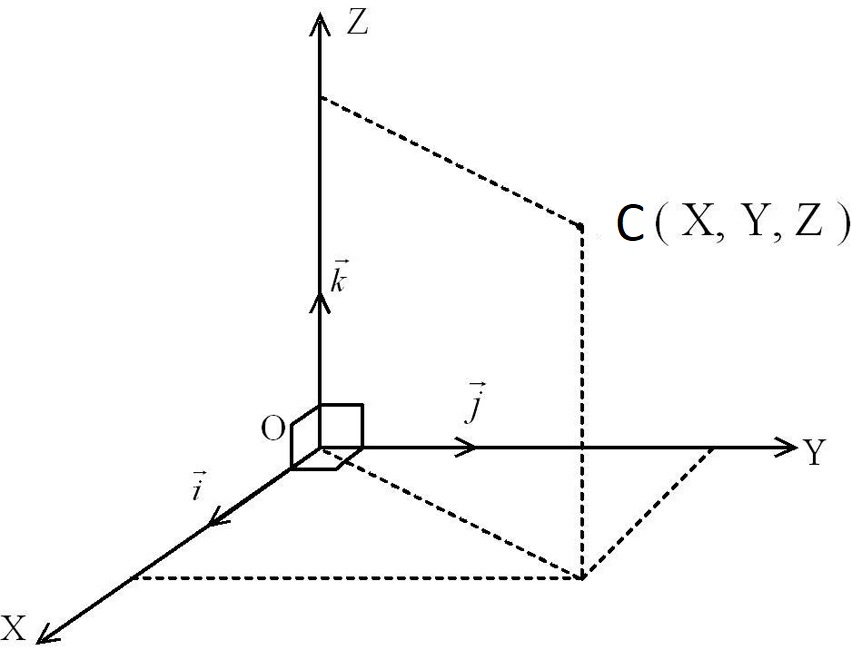
\includegraphics[width=0.6\textwidth]{R.jpg}
\caption{\label{fig:Repère R}}
\end{figure}

La force à laquelle est soumise un corps $C_{j}$ et une somme des forces gravitationnelles exercées par tout les autres corps du système. Elle s'écrit comme :

\begin{eqnarray*}
    \overrightarrow{F}_{j} &=& \sum_{i=1,i \ne j}^{N} Gm_{i}m_{j}\frac{\overrightarrow{C_{i}C_{j}}}{{|C_{i}C_{j}}|^3}
\end{eqnarray*}

On introduit ensuite notre expression de la force dans l'équation de la deuxième loi de newton :

\begin{eqnarray}
    \sum \overrightarrow{F}_{ext} &=& m\overrightarrow{a} \\
          \overrightarrow{F}_{j}  &=& m_{j}\frac{d^{2}\overrightarrow{OC}_{j}}{dt^{2}} \\
          \sum_{i=1,i \ne j}^{N} Gm_{i}\frac{\overrightarrow{C_{i}C_{j}}}{{|C_{i}C_{j}}|^3} &=& \frac{d^{2}\overrightarrow{OC}_{j}}{dt^{2}}
\end{eqnarray}

Nous avons donc une expression de l'accélération à chaque instant d'un corps $C_{j}$. En intégrant cette expression nous pouvons ainsi obtenir successivement la vitesse et la position du corps en question. C'est à cet instant que le programme entre en jeu.

\section{Partie Codage}
\label{sec:Partie Codage}

Les codes de cette partie sont dans le dossier "Headers".
\newline

On se place dans le repère du centre de masse du système. Notre code peut simuler un système à 3 dimension, mais notre but final étant de faire un jeu en 2D, nous allons donc nous limiter à 2 dimension.


\subsection{Modélisation à l'aide d'Heingen}

Notre système est modélisé comme une matrice S(m,n) avec n le nombre de corps dans le système et m deux fois le nombre dimension spatiale:

$$S = \left[\begin{matrix}
    X_1 & X_2 & \cdots & X_n\\
    Y_1 & Y_2 & \cdots & Y_n\\
    \vdots & \vdots &\cdots & \vdots\\
    V_{X1} & V_{X2} & \cdots & V_{Xn}\\
    V_{Y1} & V_{Y2} & \cdots & V_{Yn}\\
    \vdots & \vdots &\cdots & \vdots
\end{matrix}\right]$$

et un vecteur des masses du système:

$$M = \left[\begin{matrix}
    m_1 \\
    m_2 \\
    \vdots \\
    m_n\\
\end{matrix}\right]$$

On peut donc définir dans le cadre de la résolution du système à ncorps la dérivé de notre système par apport au temps, soit $\frac{dS}{dt}$. On a donc

$$\frac{dS}{dt} = \left[\begin{matrix}
    V_{X1} & V_{X2} & \cdots & V_{Xn}\\
    V_{Y1} & V_{Y2} & \cdots & V_{Yn}\\
    \vdots & \vdots &\cdots & \vdots\\
    \vec{u}_x \cdot \vec{f}(S,M) & \vec{u}_x \cdot \vec{f}(S,M) & \cdots & \vec{u}_x \cdot \vec{f}(S,M)\\
    \vec{u}_y \cdot \vec{f}(S,M) & \vec{u}_y \cdot \vec{f}(S,M) & \cdots & \vec{u}_y \cdot \vec{f}(S,M)\\
    \vdots & \vdots &\cdots & \vdots
\end{matrix}\right]$$

avec (cf l'équation (3)) :

\begin{eqnarray*}
   \vec{f}(S,M) = \sum_{i=1,i \ne j}^{N} Gm_{i}\frac{\overrightarrow{C_{i}C_{j}}}{{|C_{i}C_{j}}|^3} \\
\end{eqnarray*}
\newpage
\subsection{Méthode de Runge-Kutta}

Nous l'avons implémenté avec Heingen

\begin{figure}[h]
\centering
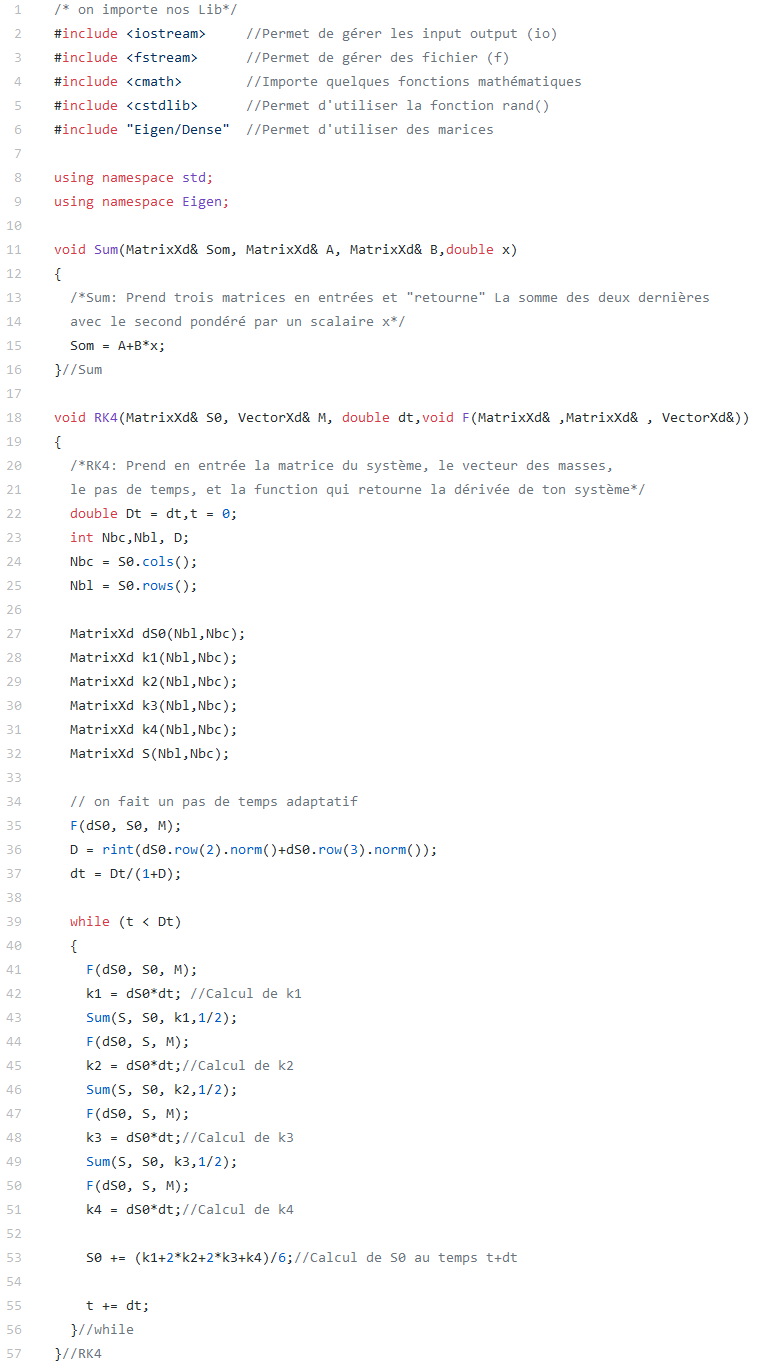
\includegraphics[width=.63\textwidth]{RK4.png}
\caption{RK4.hpp \label{fig:code}}
\end{figure}

\subsection{Le Jeu}
Le jeu nommé 2001 A Space Odyssey ou 2001ASO (en reference a l'oeuvre de Stanley Kubrick et d'Arthur C. Clarke).
Le jeu utilise le code du problème à n corps pour mettre en scène le discovery one que l'on peut guider dans le système solaire en modifiant la vitesse de celui-ci en le propulsant.
\begin{figure}[h]
\centering
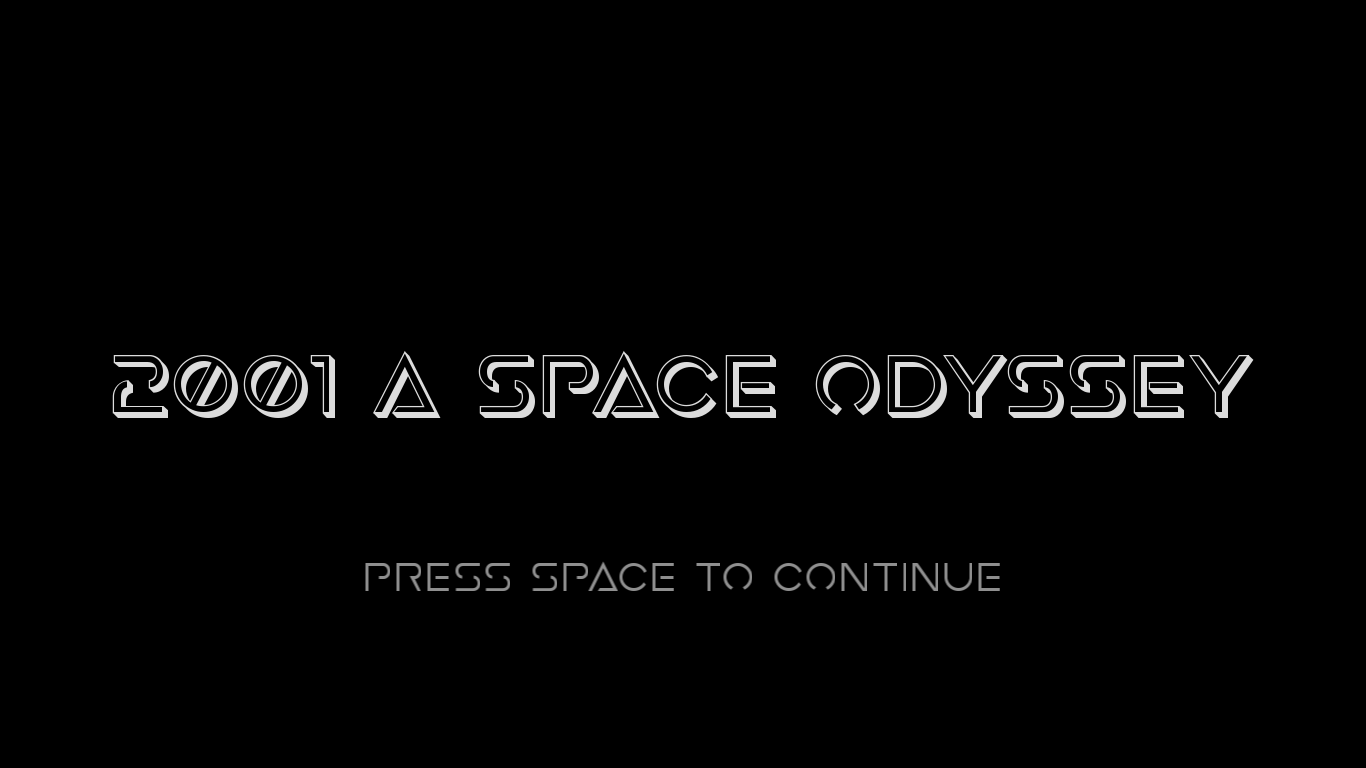
\includegraphics[width=.3\textwidth]{ecrandemarage.png}
 
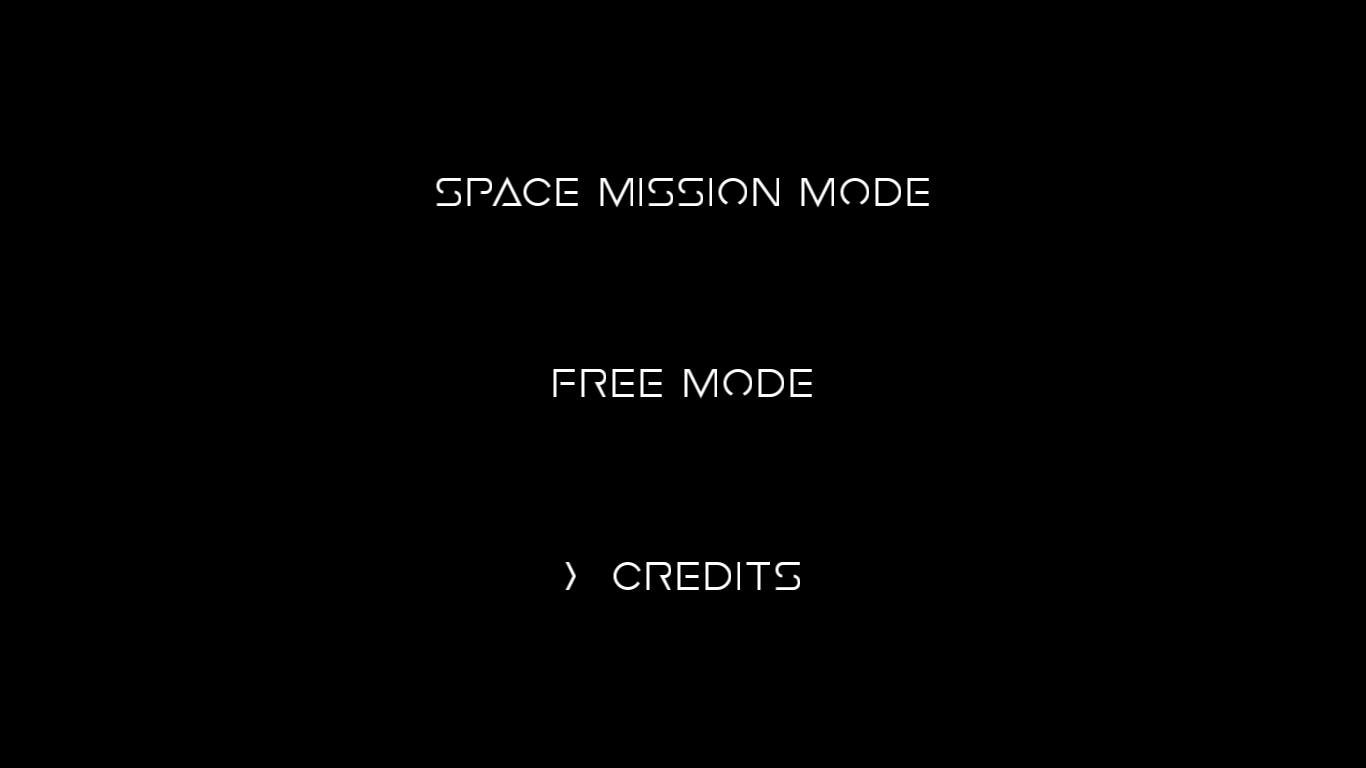
\includegraphics[width=.3\textwidth]{Choix.png}
 
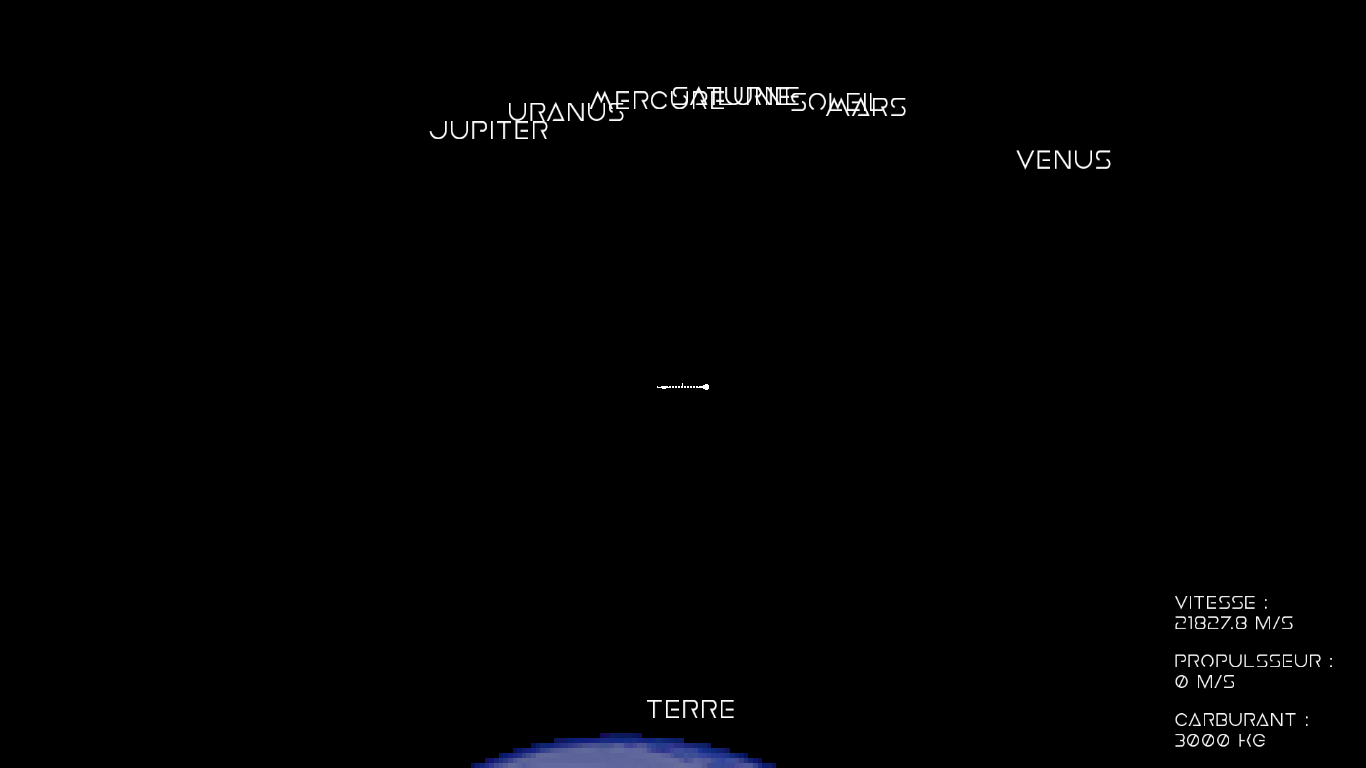
\includegraphics[width=.3\textwidth]{Jeux.png}
 
\end{figure}
Toute la partie graphique est faite grâce à la librairie SFML

Les contrôles son expliqués dans les crédits du jeu.
Deux modes jouables sont proposée.
\newpage

\section{Discussions sur les limites du modèle}
\label{sec:Discussion sur les limites du modèle}

Tout les graphes, code et scripts gnuplot de cette partie sont dans le dossier "Test".
\newline

Nous considérons un système à deux corps , tout deux ayant la masse équivalentes a celle du soleil, avec des vitesses et des distances équivalentes au système Soleil-Jupiter. Nous regardons son évolution  sur un intervalle de temps donné. (Nous avons choisi de telles conditions pour pousser à bout la simulation)

\begin{figure}[h]
\centering
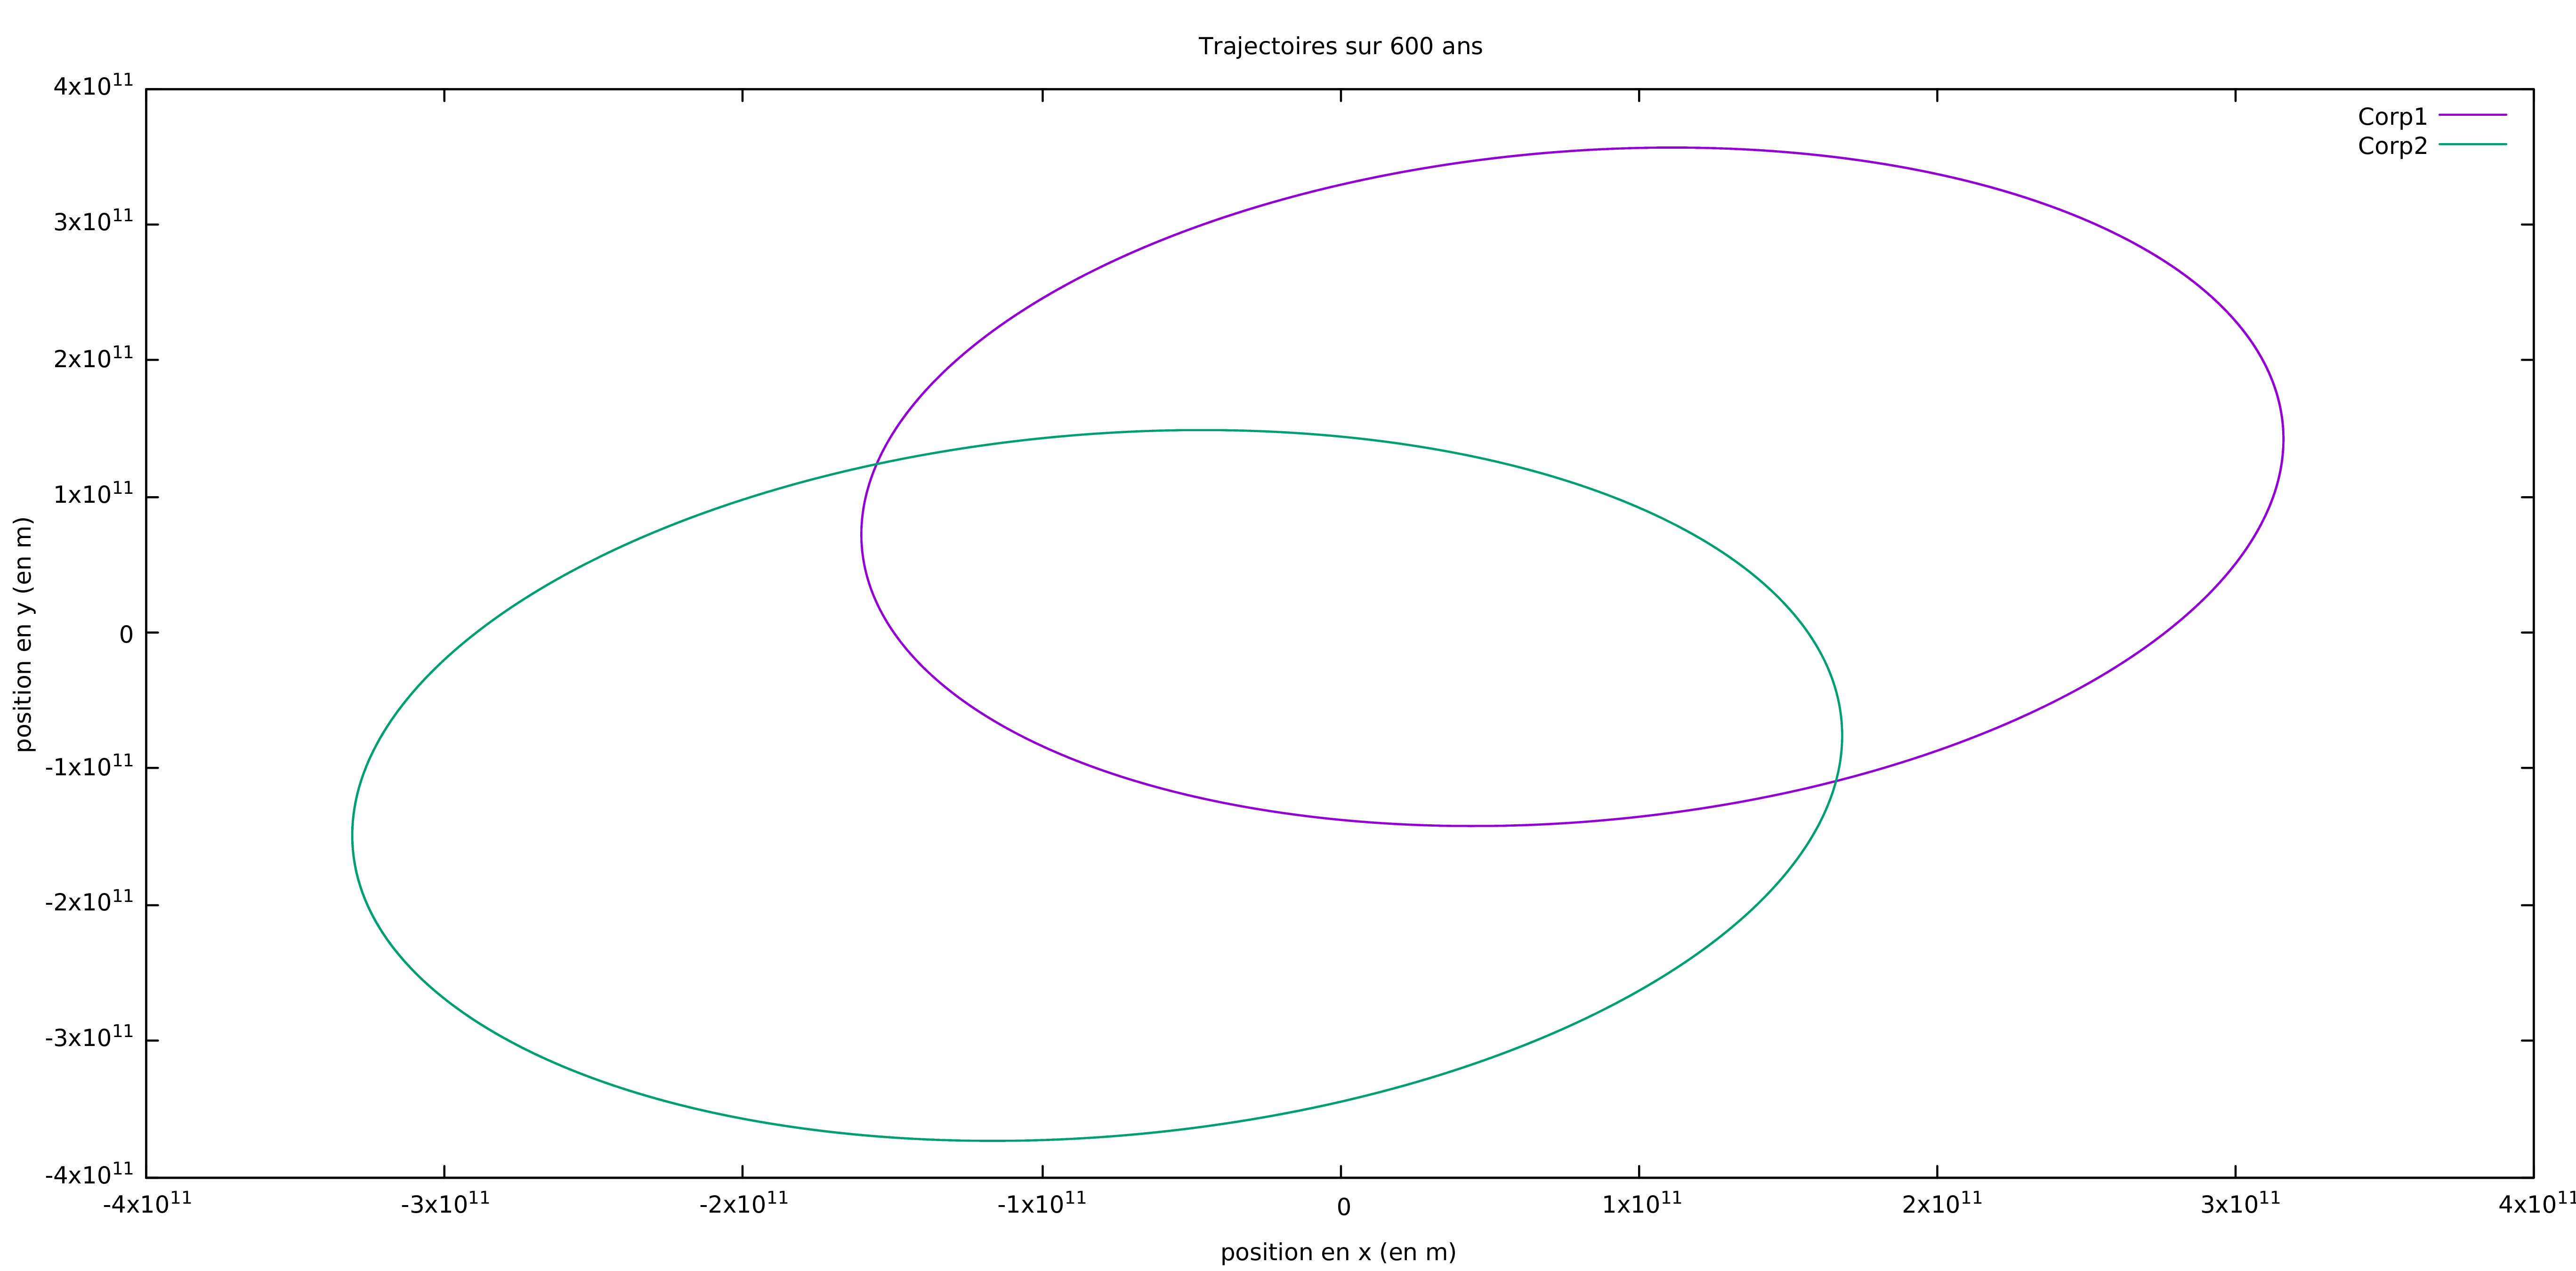
\includegraphics[width=.9\textwidth]{2.png}
\caption{Orbite des deux corps}
\end{figure}

La figure 4 nous montre l'évolution de l'énergie cinétique, l'energie potentiel et de l'energie totale dans le temps. En ordonnée nous avons l'énergie  (Joule) et en abscisse le temps (ans).

\begin{figure}[h]
\centering
\includegraphics[width=\textwidth]{1-0.png}
\caption{Evolution de l'énergie cinétique (violet), potentielle (vert) et totale (bleu) en fonction du temps.}
\end{figure}
\newpage

Jusqu'ici rien d'anormal mais si nous regardons plus en détail la dérive de l'énergie totale du système (en $E_0$ l'énérgie à $t = 0$), en fonction du temps (ans) nous avons donc une énergie totale qui augmente .

\begin{figure}[h]
\centering
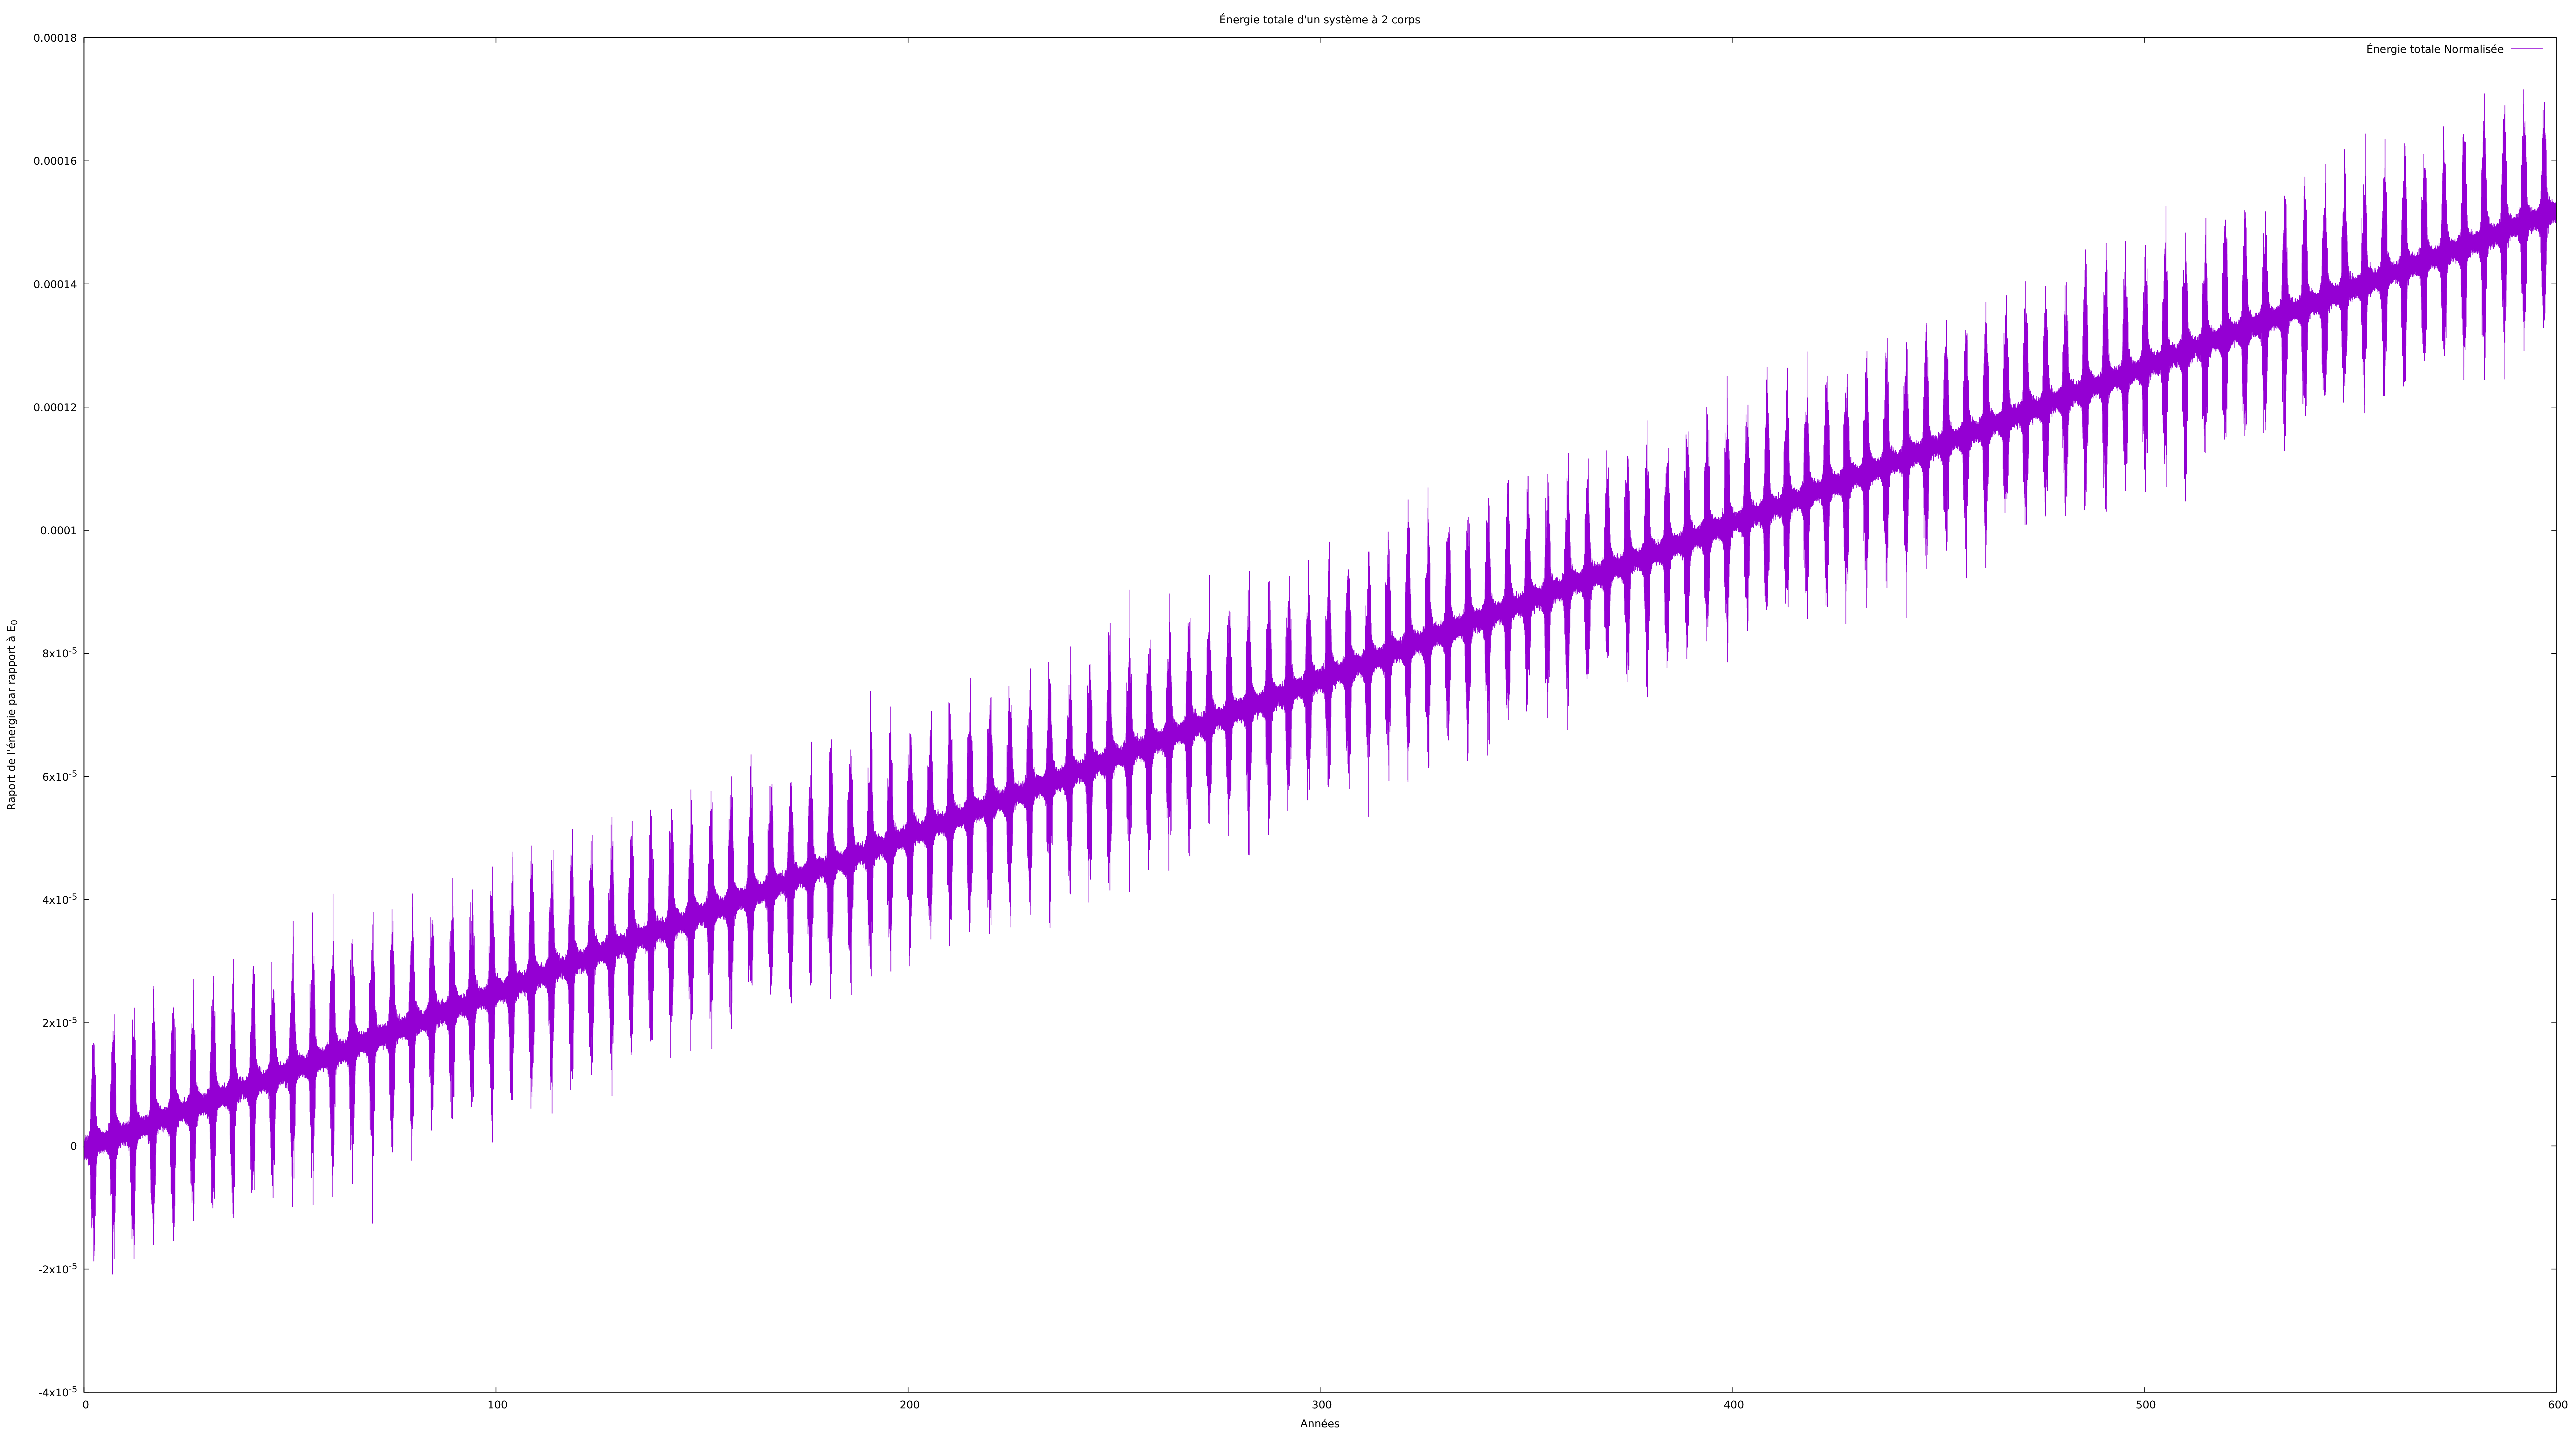
\includegraphics[width=\textwidth]{Der.png}
\caption{Evolution de l'énergie totale en fonction du temps.}
\end{figure}

En effet si l'on regarde plus près les trajectoires de deux corps nous pouvons voir que le système dérive petit à petit.

\begin{figure}[h]
\centering
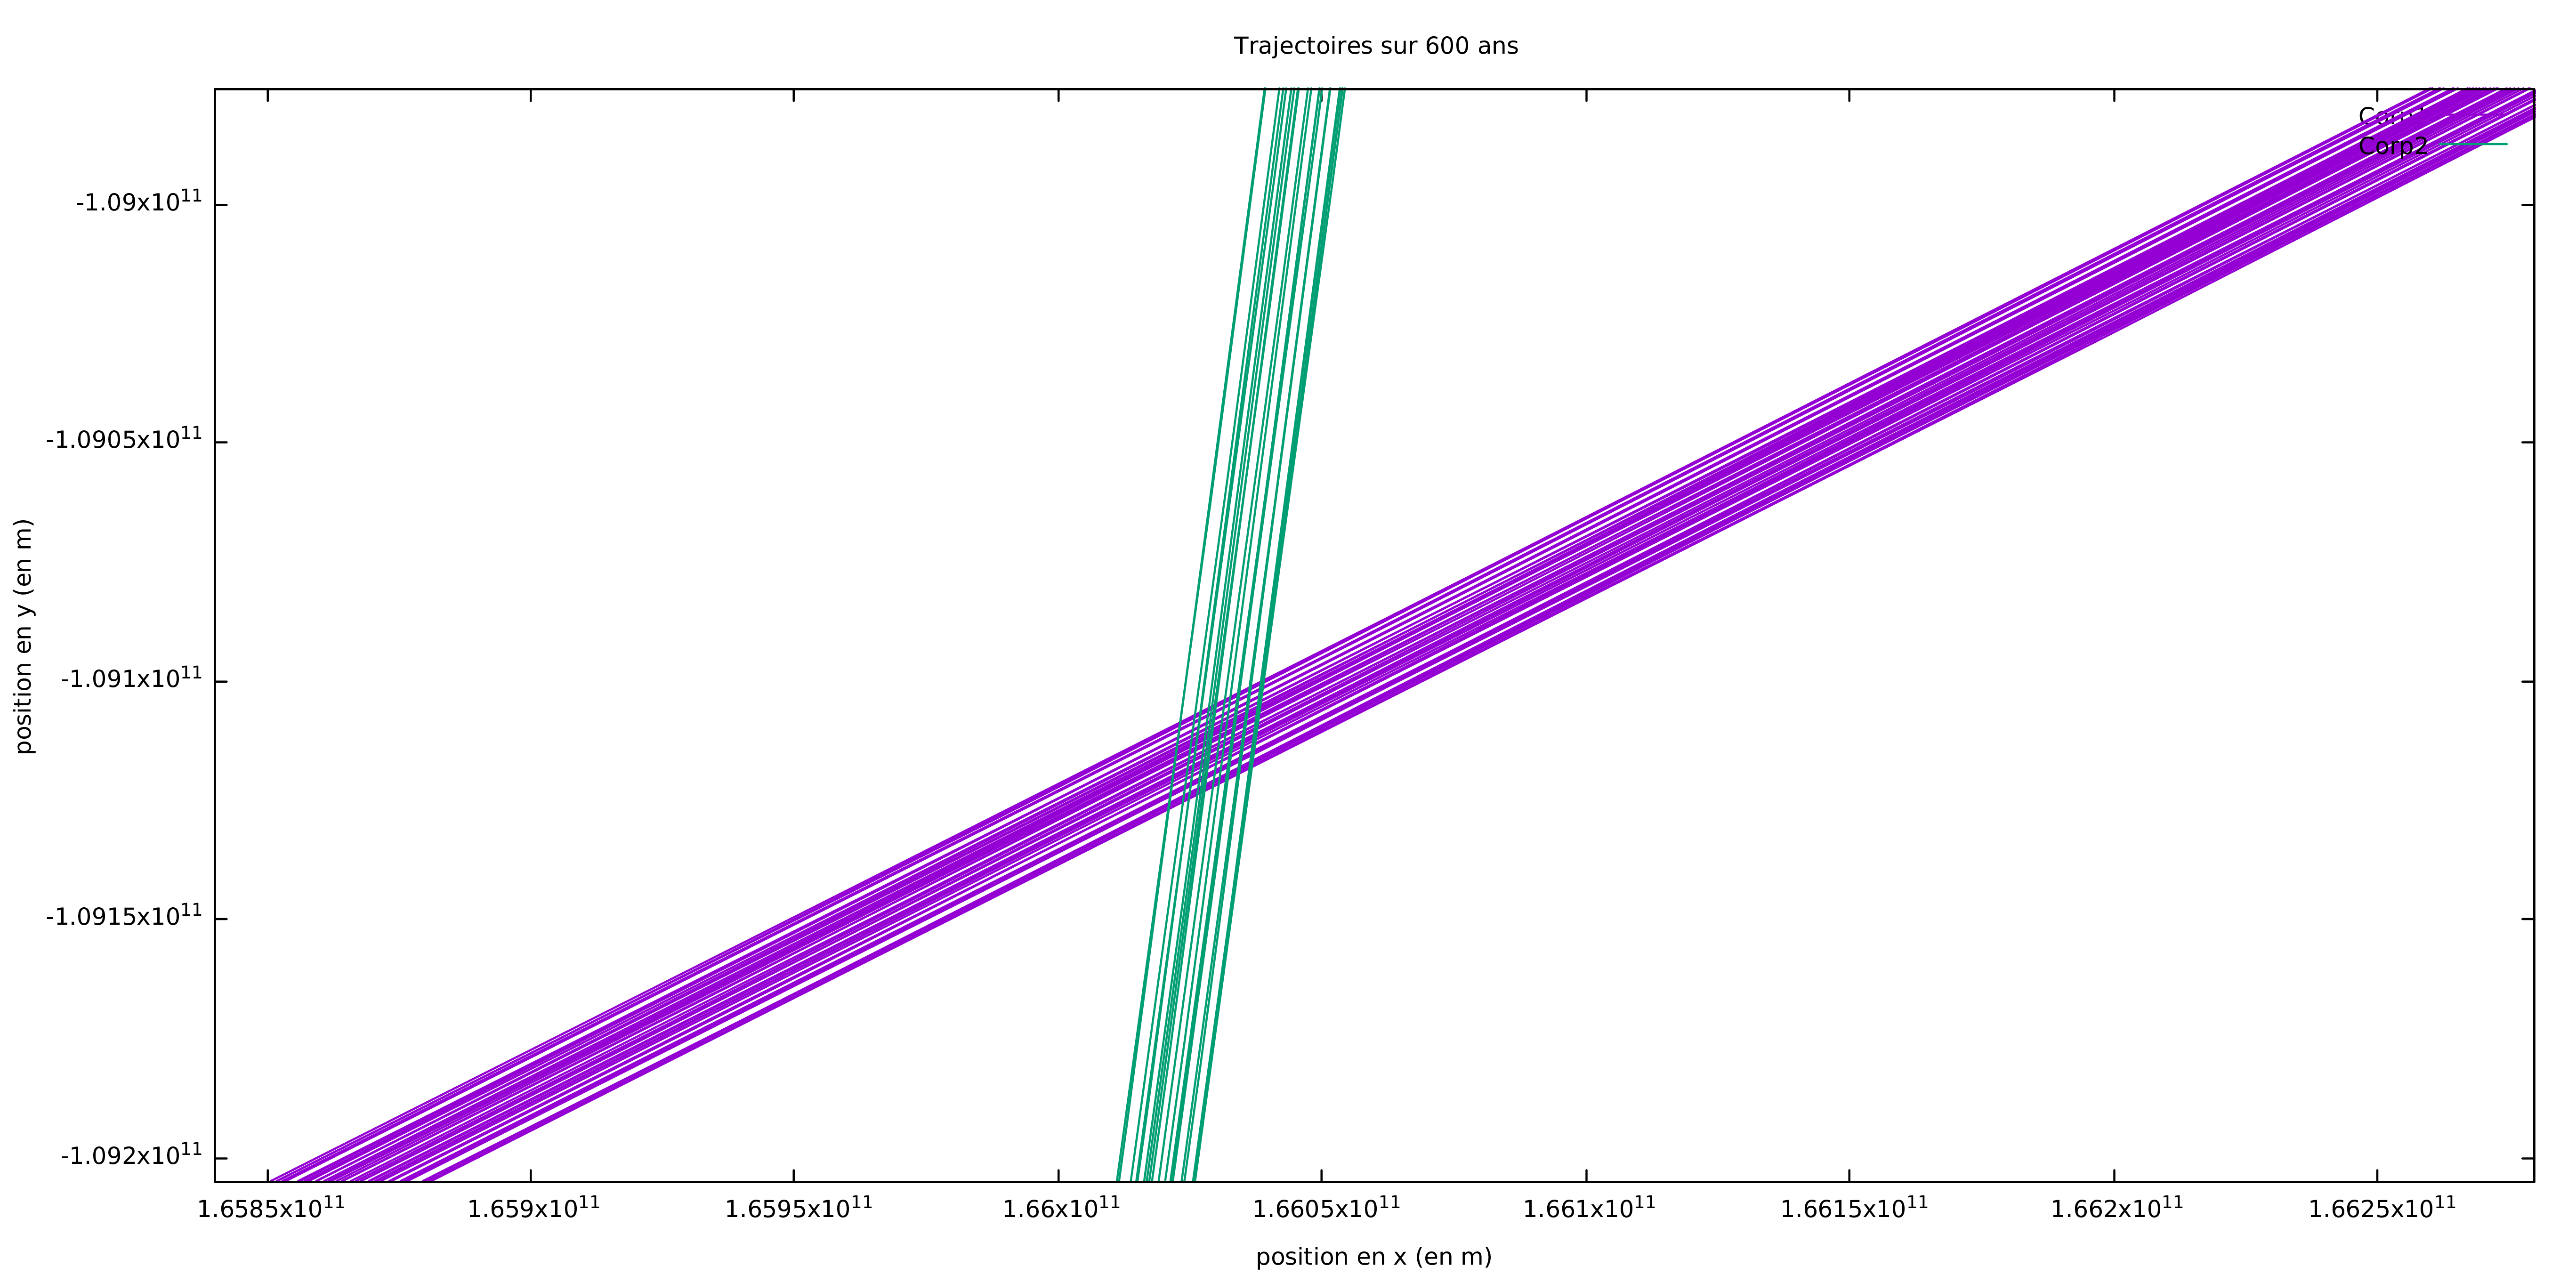
\includegraphics[width=\textwidth]{3.png}
\caption{Zoom sur la divergence des orbites des deux corps.}
\end{figure}

Nous avons donc un système qui commence à diverger au bout d'un siècle de $2 \times 10^{-5}~E_0$. Notre modèle est donc précis jusqu'à un certain point. La cause première est, comme dit plus haut (partie 2), que la méthode utilisée pour résoudre ce système bien qu'efficace est une méthode de résolution approchée.

\end{document}